
% Default to the notebook output style

    


% Inherit from the specified cell style.




    
\documentclass[11pt]{article}

    
    
    \usepackage[T1]{fontenc}
    % Nicer default font (+ math font) than Computer Modern for most use cases
    \usepackage{mathpazo}

    % Basic figure setup, for now with no caption control since it's done
    % automatically by Pandoc (which extracts ![](path) syntax from Markdown).
    \usepackage{graphicx}
    % We will generate all images so they have a width \maxwidth. This means
    % that they will get their normal width if they fit onto the page, but
    % are scaled down if they would overflow the margins.
    \makeatletter
    \def\maxwidth{\ifdim\Gin@nat@width>\linewidth\linewidth
    \else\Gin@nat@width\fi}
    \makeatother
    \let\Oldincludegraphics\includegraphics
    % Set max figure width to be 80% of text width, for now hardcoded.
    \renewcommand{\includegraphics}[1]{\Oldincludegraphics[width=.8\maxwidth]{#1}}
    % Ensure that by default, figures have no caption (until we provide a
    % proper Figure object with a Caption API and a way to capture that
    % in the conversion process - todo).
    \usepackage{caption}
    \DeclareCaptionLabelFormat{nolabel}{}
    \captionsetup{labelformat=nolabel}

    \usepackage{adjustbox} % Used to constrain images to a maximum size 
    \usepackage{xcolor} % Allow colors to be defined
    \usepackage{enumerate} % Needed for markdown enumerations to work
    \usepackage{geometry} % Used to adjust the document margins
    \usepackage{amsmath} % Equations
    \usepackage{amssymb} % Equations
    \usepackage{textcomp} % defines textquotesingle
    % Hack from http://tex.stackexchange.com/a/47451/13684:
    \AtBeginDocument{%
        \def\PYZsq{\textquotesingle}% Upright quotes in Pygmentized code
    }
    \usepackage{upquote} % Upright quotes for verbatim code
    \usepackage{eurosym} % defines \euro
    \usepackage[mathletters]{ucs} % Extended unicode (utf-8) support
    \usepackage[utf8x]{inputenc} % Allow utf-8 characters in the tex document
    \usepackage{fancyvrb} % verbatim replacement that allows latex
    \usepackage{grffile} % extends the file name processing of package graphics 
                         % to support a larger range 
    % The hyperref package gives us a pdf with properly built
    % internal navigation ('pdf bookmarks' for the table of contents,
    % internal cross-reference links, web links for URLs, etc.)
    \usepackage{hyperref}
    \usepackage{longtable} % longtable support required by pandoc >1.10
    \usepackage{booktabs}  % table support for pandoc > 1.12.2
    \usepackage[inline]{enumitem} % IRkernel/repr support (it uses the enumerate* environment)
    \usepackage[normalem]{ulem} % ulem is needed to support strikethroughs (\sout)
                                % normalem makes italics be italics, not underlines
    

    
    
    % Colors for the hyperref package
    \definecolor{urlcolor}{rgb}{0,.145,.698}
    \definecolor{linkcolor}{rgb}{.71,0.21,0.01}
    \definecolor{citecolor}{rgb}{.12,.54,.11}

    % ANSI colors
    \definecolor{ansi-black}{HTML}{3E424D}
    \definecolor{ansi-black-intense}{HTML}{282C36}
    \definecolor{ansi-red}{HTML}{E75C58}
    \definecolor{ansi-red-intense}{HTML}{B22B31}
    \definecolor{ansi-green}{HTML}{00A250}
    \definecolor{ansi-green-intense}{HTML}{007427}
    \definecolor{ansi-yellow}{HTML}{DDB62B}
    \definecolor{ansi-yellow-intense}{HTML}{B27D12}
    \definecolor{ansi-blue}{HTML}{208FFB}
    \definecolor{ansi-blue-intense}{HTML}{0065CA}
    \definecolor{ansi-magenta}{HTML}{D160C4}
    \definecolor{ansi-magenta-intense}{HTML}{A03196}
    \definecolor{ansi-cyan}{HTML}{60C6C8}
    \definecolor{ansi-cyan-intense}{HTML}{258F8F}
    \definecolor{ansi-white}{HTML}{C5C1B4}
    \definecolor{ansi-white-intense}{HTML}{A1A6B2}

    % commands and environments needed by pandoc snippets
    % extracted from the output of `pandoc -s`
    \providecommand{\tightlist}{%
      \setlength{\itemsep}{0pt}\setlength{\parskip}{0pt}}
    \DefineVerbatimEnvironment{Highlighting}{Verbatim}{commandchars=\\\{\}}
    % Add ',fontsize=\small' for more characters per line
    \newenvironment{Shaded}{}{}
    \newcommand{\KeywordTok}[1]{\textcolor[rgb]{0.00,0.44,0.13}{\textbf{{#1}}}}
    \newcommand{\DataTypeTok}[1]{\textcolor[rgb]{0.56,0.13,0.00}{{#1}}}
    \newcommand{\DecValTok}[1]{\textcolor[rgb]{0.25,0.63,0.44}{{#1}}}
    \newcommand{\BaseNTok}[1]{\textcolor[rgb]{0.25,0.63,0.44}{{#1}}}
    \newcommand{\FloatTok}[1]{\textcolor[rgb]{0.25,0.63,0.44}{{#1}}}
    \newcommand{\CharTok}[1]{\textcolor[rgb]{0.25,0.44,0.63}{{#1}}}
    \newcommand{\StringTok}[1]{\textcolor[rgb]{0.25,0.44,0.63}{{#1}}}
    \newcommand{\CommentTok}[1]{\textcolor[rgb]{0.38,0.63,0.69}{\textit{{#1}}}}
    \newcommand{\OtherTok}[1]{\textcolor[rgb]{0.00,0.44,0.13}{{#1}}}
    \newcommand{\AlertTok}[1]{\textcolor[rgb]{1.00,0.00,0.00}{\textbf{{#1}}}}
    \newcommand{\FunctionTok}[1]{\textcolor[rgb]{0.02,0.16,0.49}{{#1}}}
    \newcommand{\RegionMarkerTok}[1]{{#1}}
    \newcommand{\ErrorTok}[1]{\textcolor[rgb]{1.00,0.00,0.00}{\textbf{{#1}}}}
    \newcommand{\NormalTok}[1]{{#1}}
    
    % Additional commands for more recent versions of Pandoc
    \newcommand{\ConstantTok}[1]{\textcolor[rgb]{0.53,0.00,0.00}{{#1}}}
    \newcommand{\SpecialCharTok}[1]{\textcolor[rgb]{0.25,0.44,0.63}{{#1}}}
    \newcommand{\VerbatimStringTok}[1]{\textcolor[rgb]{0.25,0.44,0.63}{{#1}}}
    \newcommand{\SpecialStringTok}[1]{\textcolor[rgb]{0.73,0.40,0.53}{{#1}}}
    \newcommand{\ImportTok}[1]{{#1}}
    \newcommand{\DocumentationTok}[1]{\textcolor[rgb]{0.73,0.13,0.13}{\textit{{#1}}}}
    \newcommand{\AnnotationTok}[1]{\textcolor[rgb]{0.38,0.63,0.69}{\textbf{\textit{{#1}}}}}
    \newcommand{\CommentVarTok}[1]{\textcolor[rgb]{0.38,0.63,0.69}{\textbf{\textit{{#1}}}}}
    \newcommand{\VariableTok}[1]{\textcolor[rgb]{0.10,0.09,0.49}{{#1}}}
    \newcommand{\ControlFlowTok}[1]{\textcolor[rgb]{0.00,0.44,0.13}{\textbf{{#1}}}}
    \newcommand{\OperatorTok}[1]{\textcolor[rgb]{0.40,0.40,0.40}{{#1}}}
    \newcommand{\BuiltInTok}[1]{{#1}}
    \newcommand{\ExtensionTok}[1]{{#1}}
    \newcommand{\PreprocessorTok}[1]{\textcolor[rgb]{0.74,0.48,0.00}{{#1}}}
    \newcommand{\AttributeTok}[1]{\textcolor[rgb]{0.49,0.56,0.16}{{#1}}}
    \newcommand{\InformationTok}[1]{\textcolor[rgb]{0.38,0.63,0.69}{\textbf{\textit{{#1}}}}}
    \newcommand{\WarningTok}[1]{\textcolor[rgb]{0.38,0.63,0.69}{\textbf{\textit{{#1}}}}}
    
    
    % Define a nice break command that doesn't care if a line doesn't already
    % exist.
    \def\br{\hspace*{\fill} \\* }
    % Math Jax compatability definitions
    \def\gt{>}
    \def\lt{<}
    % Document parameters
    \title{MAST30032 - Biological Modelling and Simulation Semester 1 2018}
    
    
    

    % Pygments definitions
    
\makeatletter
\def\PY@reset{\let\PY@it=\relax \let\PY@bf=\relax%
    \let\PY@ul=\relax \let\PY@tc=\relax%
    \let\PY@bc=\relax \let\PY@ff=\relax}
\def\PY@tok#1{\csname PY@tok@#1\endcsname}
\def\PY@toks#1+{\ifx\relax#1\empty\else%
    \PY@tok{#1}\expandafter\PY@toks\fi}
\def\PY@do#1{\PY@bc{\PY@tc{\PY@ul{%
    \PY@it{\PY@bf{\PY@ff{#1}}}}}}}
\def\PY#1#2{\PY@reset\PY@toks#1+\relax+\PY@do{#2}}

\expandafter\def\csname PY@tok@gd\endcsname{\def\PY@tc##1{\textcolor[rgb]{0.63,0.00,0.00}{##1}}}
\expandafter\def\csname PY@tok@gu\endcsname{\let\PY@bf=\textbf\def\PY@tc##1{\textcolor[rgb]{0.50,0.00,0.50}{##1}}}
\expandafter\def\csname PY@tok@gt\endcsname{\def\PY@tc##1{\textcolor[rgb]{0.00,0.27,0.87}{##1}}}
\expandafter\def\csname PY@tok@gs\endcsname{\let\PY@bf=\textbf}
\expandafter\def\csname PY@tok@gr\endcsname{\def\PY@tc##1{\textcolor[rgb]{1.00,0.00,0.00}{##1}}}
\expandafter\def\csname PY@tok@cm\endcsname{\let\PY@it=\textit\def\PY@tc##1{\textcolor[rgb]{0.25,0.50,0.50}{##1}}}
\expandafter\def\csname PY@tok@vg\endcsname{\def\PY@tc##1{\textcolor[rgb]{0.10,0.09,0.49}{##1}}}
\expandafter\def\csname PY@tok@vi\endcsname{\def\PY@tc##1{\textcolor[rgb]{0.10,0.09,0.49}{##1}}}
\expandafter\def\csname PY@tok@vm\endcsname{\def\PY@tc##1{\textcolor[rgb]{0.10,0.09,0.49}{##1}}}
\expandafter\def\csname PY@tok@mh\endcsname{\def\PY@tc##1{\textcolor[rgb]{0.40,0.40,0.40}{##1}}}
\expandafter\def\csname PY@tok@cs\endcsname{\let\PY@it=\textit\def\PY@tc##1{\textcolor[rgb]{0.25,0.50,0.50}{##1}}}
\expandafter\def\csname PY@tok@ge\endcsname{\let\PY@it=\textit}
\expandafter\def\csname PY@tok@vc\endcsname{\def\PY@tc##1{\textcolor[rgb]{0.10,0.09,0.49}{##1}}}
\expandafter\def\csname PY@tok@il\endcsname{\def\PY@tc##1{\textcolor[rgb]{0.40,0.40,0.40}{##1}}}
\expandafter\def\csname PY@tok@go\endcsname{\def\PY@tc##1{\textcolor[rgb]{0.53,0.53,0.53}{##1}}}
\expandafter\def\csname PY@tok@cp\endcsname{\def\PY@tc##1{\textcolor[rgb]{0.74,0.48,0.00}{##1}}}
\expandafter\def\csname PY@tok@gi\endcsname{\def\PY@tc##1{\textcolor[rgb]{0.00,0.63,0.00}{##1}}}
\expandafter\def\csname PY@tok@gh\endcsname{\let\PY@bf=\textbf\def\PY@tc##1{\textcolor[rgb]{0.00,0.00,0.50}{##1}}}
\expandafter\def\csname PY@tok@ni\endcsname{\let\PY@bf=\textbf\def\PY@tc##1{\textcolor[rgb]{0.60,0.60,0.60}{##1}}}
\expandafter\def\csname PY@tok@nl\endcsname{\def\PY@tc##1{\textcolor[rgb]{0.63,0.63,0.00}{##1}}}
\expandafter\def\csname PY@tok@nn\endcsname{\let\PY@bf=\textbf\def\PY@tc##1{\textcolor[rgb]{0.00,0.00,1.00}{##1}}}
\expandafter\def\csname PY@tok@no\endcsname{\def\PY@tc##1{\textcolor[rgb]{0.53,0.00,0.00}{##1}}}
\expandafter\def\csname PY@tok@na\endcsname{\def\PY@tc##1{\textcolor[rgb]{0.49,0.56,0.16}{##1}}}
\expandafter\def\csname PY@tok@nb\endcsname{\def\PY@tc##1{\textcolor[rgb]{0.00,0.50,0.00}{##1}}}
\expandafter\def\csname PY@tok@nc\endcsname{\let\PY@bf=\textbf\def\PY@tc##1{\textcolor[rgb]{0.00,0.00,1.00}{##1}}}
\expandafter\def\csname PY@tok@nd\endcsname{\def\PY@tc##1{\textcolor[rgb]{0.67,0.13,1.00}{##1}}}
\expandafter\def\csname PY@tok@ne\endcsname{\let\PY@bf=\textbf\def\PY@tc##1{\textcolor[rgb]{0.82,0.25,0.23}{##1}}}
\expandafter\def\csname PY@tok@nf\endcsname{\def\PY@tc##1{\textcolor[rgb]{0.00,0.00,1.00}{##1}}}
\expandafter\def\csname PY@tok@si\endcsname{\let\PY@bf=\textbf\def\PY@tc##1{\textcolor[rgb]{0.73,0.40,0.53}{##1}}}
\expandafter\def\csname PY@tok@s2\endcsname{\def\PY@tc##1{\textcolor[rgb]{0.73,0.13,0.13}{##1}}}
\expandafter\def\csname PY@tok@nt\endcsname{\let\PY@bf=\textbf\def\PY@tc##1{\textcolor[rgb]{0.00,0.50,0.00}{##1}}}
\expandafter\def\csname PY@tok@nv\endcsname{\def\PY@tc##1{\textcolor[rgb]{0.10,0.09,0.49}{##1}}}
\expandafter\def\csname PY@tok@s1\endcsname{\def\PY@tc##1{\textcolor[rgb]{0.73,0.13,0.13}{##1}}}
\expandafter\def\csname PY@tok@dl\endcsname{\def\PY@tc##1{\textcolor[rgb]{0.73,0.13,0.13}{##1}}}
\expandafter\def\csname PY@tok@ch\endcsname{\let\PY@it=\textit\def\PY@tc##1{\textcolor[rgb]{0.25,0.50,0.50}{##1}}}
\expandafter\def\csname PY@tok@m\endcsname{\def\PY@tc##1{\textcolor[rgb]{0.40,0.40,0.40}{##1}}}
\expandafter\def\csname PY@tok@gp\endcsname{\let\PY@bf=\textbf\def\PY@tc##1{\textcolor[rgb]{0.00,0.00,0.50}{##1}}}
\expandafter\def\csname PY@tok@sh\endcsname{\def\PY@tc##1{\textcolor[rgb]{0.73,0.13,0.13}{##1}}}
\expandafter\def\csname PY@tok@ow\endcsname{\let\PY@bf=\textbf\def\PY@tc##1{\textcolor[rgb]{0.67,0.13,1.00}{##1}}}
\expandafter\def\csname PY@tok@sx\endcsname{\def\PY@tc##1{\textcolor[rgb]{0.00,0.50,0.00}{##1}}}
\expandafter\def\csname PY@tok@bp\endcsname{\def\PY@tc##1{\textcolor[rgb]{0.00,0.50,0.00}{##1}}}
\expandafter\def\csname PY@tok@c1\endcsname{\let\PY@it=\textit\def\PY@tc##1{\textcolor[rgb]{0.25,0.50,0.50}{##1}}}
\expandafter\def\csname PY@tok@fm\endcsname{\def\PY@tc##1{\textcolor[rgb]{0.00,0.00,1.00}{##1}}}
\expandafter\def\csname PY@tok@o\endcsname{\def\PY@tc##1{\textcolor[rgb]{0.40,0.40,0.40}{##1}}}
\expandafter\def\csname PY@tok@kc\endcsname{\let\PY@bf=\textbf\def\PY@tc##1{\textcolor[rgb]{0.00,0.50,0.00}{##1}}}
\expandafter\def\csname PY@tok@c\endcsname{\let\PY@it=\textit\def\PY@tc##1{\textcolor[rgb]{0.25,0.50,0.50}{##1}}}
\expandafter\def\csname PY@tok@mf\endcsname{\def\PY@tc##1{\textcolor[rgb]{0.40,0.40,0.40}{##1}}}
\expandafter\def\csname PY@tok@err\endcsname{\def\PY@bc##1{\setlength{\fboxsep}{0pt}\fcolorbox[rgb]{1.00,0.00,0.00}{1,1,1}{\strut ##1}}}
\expandafter\def\csname PY@tok@mb\endcsname{\def\PY@tc##1{\textcolor[rgb]{0.40,0.40,0.40}{##1}}}
\expandafter\def\csname PY@tok@ss\endcsname{\def\PY@tc##1{\textcolor[rgb]{0.10,0.09,0.49}{##1}}}
\expandafter\def\csname PY@tok@sr\endcsname{\def\PY@tc##1{\textcolor[rgb]{0.73,0.40,0.53}{##1}}}
\expandafter\def\csname PY@tok@mo\endcsname{\def\PY@tc##1{\textcolor[rgb]{0.40,0.40,0.40}{##1}}}
\expandafter\def\csname PY@tok@kd\endcsname{\let\PY@bf=\textbf\def\PY@tc##1{\textcolor[rgb]{0.00,0.50,0.00}{##1}}}
\expandafter\def\csname PY@tok@mi\endcsname{\def\PY@tc##1{\textcolor[rgb]{0.40,0.40,0.40}{##1}}}
\expandafter\def\csname PY@tok@kn\endcsname{\let\PY@bf=\textbf\def\PY@tc##1{\textcolor[rgb]{0.00,0.50,0.00}{##1}}}
\expandafter\def\csname PY@tok@cpf\endcsname{\let\PY@it=\textit\def\PY@tc##1{\textcolor[rgb]{0.25,0.50,0.50}{##1}}}
\expandafter\def\csname PY@tok@kr\endcsname{\let\PY@bf=\textbf\def\PY@tc##1{\textcolor[rgb]{0.00,0.50,0.00}{##1}}}
\expandafter\def\csname PY@tok@s\endcsname{\def\PY@tc##1{\textcolor[rgb]{0.73,0.13,0.13}{##1}}}
\expandafter\def\csname PY@tok@kp\endcsname{\def\PY@tc##1{\textcolor[rgb]{0.00,0.50,0.00}{##1}}}
\expandafter\def\csname PY@tok@w\endcsname{\def\PY@tc##1{\textcolor[rgb]{0.73,0.73,0.73}{##1}}}
\expandafter\def\csname PY@tok@kt\endcsname{\def\PY@tc##1{\textcolor[rgb]{0.69,0.00,0.25}{##1}}}
\expandafter\def\csname PY@tok@sc\endcsname{\def\PY@tc##1{\textcolor[rgb]{0.73,0.13,0.13}{##1}}}
\expandafter\def\csname PY@tok@sb\endcsname{\def\PY@tc##1{\textcolor[rgb]{0.73,0.13,0.13}{##1}}}
\expandafter\def\csname PY@tok@sa\endcsname{\def\PY@tc##1{\textcolor[rgb]{0.73,0.13,0.13}{##1}}}
\expandafter\def\csname PY@tok@k\endcsname{\let\PY@bf=\textbf\def\PY@tc##1{\textcolor[rgb]{0.00,0.50,0.00}{##1}}}
\expandafter\def\csname PY@tok@se\endcsname{\let\PY@bf=\textbf\def\PY@tc##1{\textcolor[rgb]{0.73,0.40,0.13}{##1}}}
\expandafter\def\csname PY@tok@sd\endcsname{\let\PY@it=\textit\def\PY@tc##1{\textcolor[rgb]{0.73,0.13,0.13}{##1}}}

\def\PYZbs{\char`\\}
\def\PYZus{\char`\_}
\def\PYZob{\char`\{}
\def\PYZcb{\char`\}}
\def\PYZca{\char`\^}
\def\PYZam{\char`\&}
\def\PYZlt{\char`\<}
\def\PYZgt{\char`\>}
\def\PYZsh{\char`\#}
\def\PYZpc{\char`\%}
\def\PYZdl{\char`\$}
\def\PYZhy{\char`\-}
\def\PYZsq{\char`\'}
\def\PYZdq{\char`\"}
\def\PYZti{\char`\~}
% for compatibility with earlier versions
\def\PYZat{@}
\def\PYZlb{[}
\def\PYZrb{]}
\makeatother


    % Exact colors from NB
    \definecolor{incolor}{rgb}{0.0, 0.0, 0.5}
    \definecolor{outcolor}{rgb}{0.545, 0.0, 0.0}



    
    % Prevent overflowing lines due to hard-to-break entities
    \sloppy 
    % Setup hyperref package
    \hypersetup{
      breaklinks=true,  % so long urls are correctly broken across lines
      colorlinks=true,
      urlcolor=urlcolor,
      linkcolor=linkcolor,
      citecolor=citecolor,
      }
    % Slightly bigger margins than the latex defaults
    
    \geometry{verbose,tmargin=1in,bmargin=1in,lmargin=1in,rmargin=1in}
    
    

    \begin{document}
    
    
    \maketitle
    
    

    
    \section{MAST30032: Biological Modelling and
Simulation}\label{mast30032-biological-modelling-and-simulation}

Author: Stephen Zhang

    \subsection{Discrete-time models}\label{discrete-time-models}

Discrete-time models in general concern \emph{difference equations}. We
will focus on \emph{first order} difference equations, which describe
sequences \(\{x_n\}\) such that:

\[x_{n+1} \leftarrow f(x_n)\]

The function \(f(\cdot)\) is called the \emph{map}.

\subsubsection{Solution of first-order linear difference
equations}\label{solution-of-first-order-linear-difference-equations}

Consider an equation with the general form

\[x_{n+1} = ax_n + P(x), a \in \mathbb{R}\]

We rewrite this as \(x_{n+1} - ax_n = P(n)\), then split into
\emph{homogeneous} and \emph{inhomogeneous} equations:

\begin{align}
    x_{n+1} - ax_n &= 0 \quad &\text{homogeneous}\\
    x_{n+1} - ax_n &= P(n) \quad &\text{inhomogeneous}\\
\end{align}

A simple solution (verify this) of the homogeneous solution is
\({x_n}^h = Ca^n\). We need to \textbf{guess} some \(Q(n)\), a solution
to the inhomogeneous equation.

The \textbf{overall} solution is given by superposition:

\[x_n = {x_n}^h + {x_n}^i = Ca^n + Q(n)\]

\subsubsection{\texorpdfstring{Behaviour of systems of the form
\(x_{n+1} = rx_n\)}{Behaviour of systems of the form x\_\{n+1\} = rx\_n}}\label{behaviour-of-systems-of-the-form-xux5fn1-rxux5fn}

Consider the case \(x_{n+1} = rx_n\) which has solution
\(x_n = r^tx_0\). There are \textbf{seven} classes

\begin{enumerate}
\def\labelenumi{\arabic{enumi}.}
\tightlist
\item
  \(r = 0\): solution is zero except possibly \(x_0\)
\item
  \(r = 1\): solution is constant everywhere
\item
  \(r = -1\): solution oscillates between \(+x_0\) and \(-x_0\)
\item
  \(r \in (0, 1)\): \(x_n \to 0\) as \(n \to \infty\) monotonically
\item
  \(r \in (-1, 0)\): \(x_n \to 0\) as \(n \to \infty\) by bounded
  oscillation
\item
  \(r > 1\): \(x_n \to \infty\) as \(n \to \infty\) monotonically
\item
  \(r < -1\): \(|x_n| \to \infty\) as \(n \to \infty\) and \(x_n\)
  oscillates unboundedly
\end{enumerate}

\subsubsection{Analysis by cobwebbing}\label{analysis-by-cobwebbing}

Cobwebbing is a graphical method for determining the long-term behaviour
of a discrete dynamical system. Consider the general case
\(x_{n+1} = f(x_n)\). Fixed points of our system are solutions of
\(x = f(x)\).

That is, they will be the intersection between the graph of \(y = f(x)\)
and \(y = x\).

\begin{figure}[htbp]
\centering
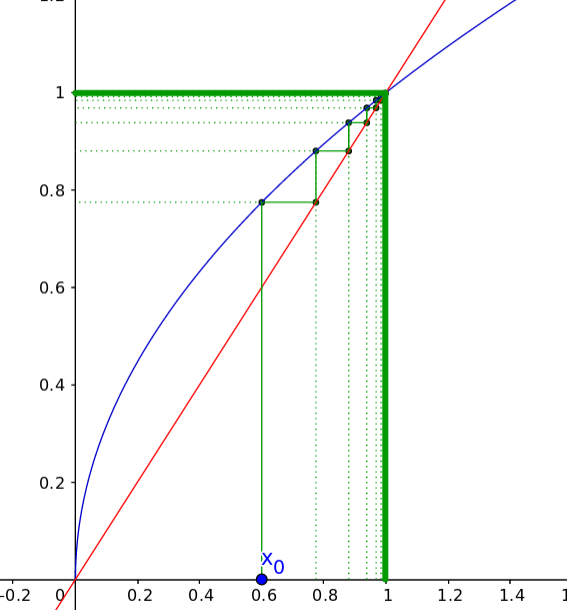
\includegraphics{cobweb1.png}
\caption{Cobweb of \(y = \sqrt{x}\) , \(x_0 = 0.6\)}
\end{figure}

Here, we see the cobweb of \(x_{n+1} = \sqrt{x}\) starting from
\(x_0 = 0.6\). Observe that we converge towards \(x = 1\), one of the
fixed points of our dynamical system. We call \(x = 1\) \textbf{stable},
because starting from \(x = 0.6\) results in attraction to \(x = 1\). On
the other hand, \(x = 0\) is an \textbf{unstable} fixed point, since
starting close to \(x = 0\) will result in repulsion (see below).

\begin{figure}[htbp]
\centering
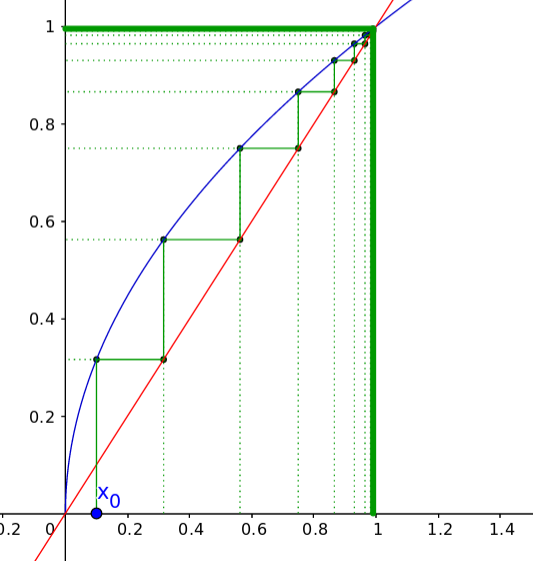
\includegraphics{cobweb2.png}
\caption{}
\end{figure}

Cobwebbing can show us situations that result in oscillatory behaviour
around a fixed point, such as when \(f(x) = 1-0.5x^2\) and
\(x_0 = 0.91\):

\begin{figure}[htbp]
\centering
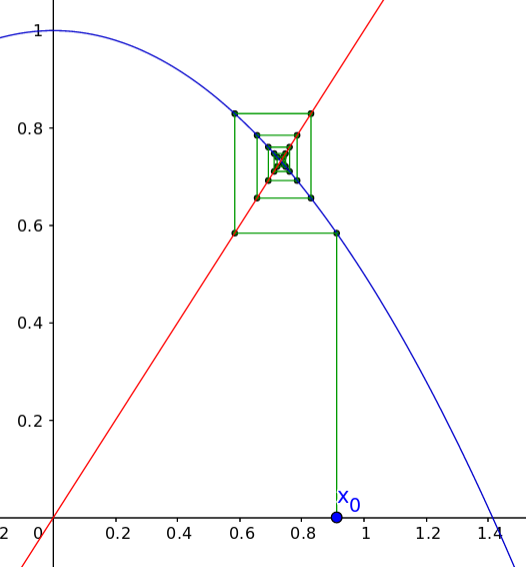
\includegraphics{cobweb3.png}
\caption{}
\end{figure}

The results observed from cobwebbing are formalised as \emph{linear
stability analysis}.

\subsubsection{General linear stability
analysis}\label{general-linear-stability-analysis}

Consider the dynamical system described by:

\[u_{t+1} = f(u_t ; r)\]

Here, \(r\) is some parameter in the model (its importance will show
later!)

Let us first determine the \emph{stable (fixed) points} of our system -
such points are solutions to the equation \(u = f(u; r)\). Let \(u^*\)
be such a stable point.

Clearly, if \(u_0 = u^*\) then \(u_t = u^*\) everywhere. This is not
interesting - we want to know about the behaviour of our system
\emph{close} to \(u^*\). Let us thus consider some perturbation
\(\delta_n\) away from our fixed point - we would like to know the
\emph{fate} of this perturbation as it propagates with the evolution of
time in our system.

Consider using the Taylor series expansion:

\begin{align}
    u^* + \delta_{n+1} &= f(u^* + \delta_n; r)\\
    &= f(u^*) + \delta_nf'(u^*) + \mathcal{O}(\delta_n^2)
\end{align}

Since \(\delta_n \ll 1\), we have

\[u^* + \delta_{n+1} = \underbrace{(u^*)}_{ = u^*} + \delta_nf'(u^*)\]

Thus

\[\delta_{n+1} = f'(u^*)\delta_n\]

*** Eigenvalues of steady states***

We call \(\lambda = f'(u^*)\) the \emph{eigenvalue} of the system
associated with the steady state \(u^*\).

Clearly, if \(|\lambda| < 1\), then \(\delta_{n} \to 0\) as
\(n \to \infty\); that is, \(u^*\) is said to be stable. * Specifically,
if \(-1 < \lambda < 0\), we obtain \emph{oscillatory} behaviour.

Consider the case \(\lambda = \pm 1\). This corresponds to the points in
our parameter space where the nature of our steady state \emph{changes}.

Consider the \textbf{quadratic map} specified by \(f(x) = rx(1-x)\).

Solving for steady states, we obtain:

\begin{align*}
    x^*_1 &= 0\\
    x^*_2 &= 1 - \dfrac{1}{r}\\
\end{align*}

Compute the derivative at these points using
\(f'(x) = r\left( 1-x\right) -rx\)

\begin{align*}
    f'(x^*_1) &= r\\
    f'(x^*_2) &= 2-r
\end{align*}

\(x^*_1 = 0\) is stable for \(|r| < 1\). \(x^*_2 = 1 - 1/r\) is stable
for \(1<r<3\). We can thus plot the \textbf{stable} solutions to our
system as a function of \(r\).

    \begin{Verbatim}[commandchars=\\\{\}]
{\color{incolor}In [{\color{incolor}4}]:} \PY{k+kn}{import} \PY{n+nn}{matplotlib} \PY{k+kn}{as} \PY{n+nn}{mp}
        \PY{k+kn}{import} \PY{n+nn}{matplotlib.pyplot} \PY{k+kn}{as} \PY{n+nn}{plt}
        \PY{n}{plt}\PY{o}{.}\PY{n}{figure}\PY{p}{(}\PY{p}{)}
        \PY{n}{x} \PY{o}{=} \PY{p}{[}\PY{l+m+mf}{0.01}\PY{o}{*}\PY{n}{i} \PY{k}{for} \PY{n}{i} \PY{o+ow}{in} \PY{n+nb}{range}\PY{p}{(}\PY{l+m+mi}{0}\PY{p}{,} \PY{l+m+mi}{300}\PY{p}{)}\PY{p}{]}
        \PY{n}{y} \PY{o}{=} \PY{p}{[}\PY{l+m+mi}{0} \PY{k}{for} \PY{n}{i} \PY{o+ow}{in} \PY{n+nb}{range}\PY{p}{(}\PY{l+m+mi}{0}\PY{p}{,} \PY{l+m+mi}{100}\PY{p}{)}\PY{p}{]} \PY{o}{+} \PY{p}{[}\PY{l+m+mi}{1} \PY{o}{\PYZhy{}} \PY{l+m+mi}{1}\PY{o}{/}\PY{p}{(}\PY{l+m+mf}{0.01}\PY{o}{*}\PY{n}{i}\PY{p}{)} \PY{k}{for} \PY{n}{i} \PY{o+ow}{in} \PY{n+nb}{range}\PY{p}{(}\PY{l+m+mi}{100}\PY{p}{,} \PY{l+m+mi}{300}\PY{p}{)}\PY{p}{]}
        \PY{n}{plt}\PY{o}{.}\PY{n}{plot}\PY{p}{(}\PY{n}{x}\PY{p}{,} \PY{n}{y}\PY{p}{)}
        \PY{n}{plt}\PY{o}{.}\PY{n}{title}\PY{p}{(}\PY{l+s+s2}{\PYZdq{}}\PY{l+s+s2}{Plot of stable fixed points for map \PYZdl{}f(x) = rx(1\PYZhy{}x)\PYZdl{} for \PYZdl{}r }\PY{l+s+s2}{\PYZbs{}}\PY{l+s+s2}{in [0, 3]\PYZdl{}}\PY{l+s+s2}{\PYZdq{}}\PY{p}{)}
\end{Verbatim}


\begin{Verbatim}[commandchars=\\\{\}]
{\color{outcolor}Out[{\color{outcolor}4}]:} Text(0.5,1,'Plot of stable fixed points for map \$f(x) = rx(1-x)\$ for \$r \textbackslash{}\textbackslash{}in [0, 3]\$')
\end{Verbatim}
            
    \begin{center}
    \adjustimage{max size={0.9\linewidth}{0.9\paperheight}}{output_2_1.png}
    \end{center}
    { \hspace*{\fill} \\}
    
    \begin{Verbatim}[commandchars=\\\{\}]
{\color{incolor}In [{\color{incolor}5}]:} \PY{k+kn}{from} \PY{n+nn}{iterate} \PY{k+kn}{import} \PY{n}{iterate}
        \PY{n}{r} \PY{o}{=} \PY{l+m+mf}{0.5}
        \PY{n}{x} \PY{o}{=} \PY{n}{iterate}\PY{p}{(}\PY{l+m+mi}{30}\PY{p}{,} \PY{k}{lambda} \PY{n}{x}\PY{p}{:} \PY{n}{r}\PY{o}{*}\PY{n}{x}\PY{o}{*}\PY{p}{(}\PY{l+m+mi}{1}\PY{o}{\PYZhy{}}\PY{n}{x}\PY{p}{)}\PY{p}{,} \PY{n}{x0} \PY{o}{=} \PY{l+m+mf}{0.5}\PY{p}{)}
        
        \PY{n}{plt}\PY{o}{.}\PY{n}{figure}\PY{p}{(}\PY{p}{)}
        \PY{n}{plt}\PY{o}{.}\PY{n}{scatter}\PY{p}{(}\PY{p}{[}\PY{n}{i}\PY{p}{[}\PY{l+m+mi}{0}\PY{p}{]} \PY{k}{for} \PY{n}{i} \PY{o+ow}{in} \PY{n}{x}\PY{p}{]}\PY{p}{,} \PY{p}{[}\PY{n}{i}\PY{p}{[}\PY{l+m+mi}{1}\PY{p}{]} \PY{k}{for} \PY{n}{i} \PY{o+ow}{in} \PY{n}{x}\PY{p}{]}\PY{p}{)}
        \PY{n}{plt}\PY{o}{.}\PY{n}{title}\PY{p}{(}\PY{l+s+s2}{\PYZdq{}}\PY{l+s+s2}{Plot of iterative solution with r = 0.5}\PY{l+s+s2}{\PYZdq{}}\PY{p}{)}
        \PY{n}{plt}\PY{o}{.}\PY{n}{ylim}\PY{p}{(}\PY{o}{\PYZhy{}}\PY{l+m+mf}{0.1}\PY{p}{,} \PY{l+m+mi}{1}\PY{p}{)}
        
        \PY{n}{r} \PY{o}{=} \PY{l+m+mf}{1.5}
        \PY{n}{x} \PY{o}{=} \PY{n}{iterate}\PY{p}{(}\PY{l+m+mi}{30}\PY{p}{,} \PY{k}{lambda} \PY{n}{x}\PY{p}{:} \PY{n}{r}\PY{o}{*}\PY{n}{x}\PY{o}{*}\PY{p}{(}\PY{l+m+mi}{1}\PY{o}{\PYZhy{}}\PY{n}{x}\PY{p}{)}\PY{p}{,} \PY{n}{x0} \PY{o}{=} \PY{l+m+mf}{0.01}\PY{p}{)}
        \PY{n}{plt}\PY{o}{.}\PY{n}{figure}\PY{p}{(}\PY{p}{)}
        \PY{n}{plt}\PY{o}{.}\PY{n}{scatter}\PY{p}{(}\PY{p}{[}\PY{n}{i}\PY{p}{[}\PY{l+m+mi}{0}\PY{p}{]} \PY{k}{for} \PY{n}{i} \PY{o+ow}{in} \PY{n}{x}\PY{p}{]}\PY{p}{,} \PY{p}{[}\PY{n}{i}\PY{p}{[}\PY{l+m+mi}{1}\PY{p}{]} \PY{k}{for} \PY{n}{i} \PY{o+ow}{in} \PY{n}{x}\PY{p}{]}\PY{p}{)}
        \PY{n}{plt}\PY{o}{.}\PY{n}{ylim}\PY{p}{(}\PY{l+m+mi}{0}\PY{p}{,} \PY{l+m+mi}{1}\PY{p}{)}
        \PY{n}{plt}\PY{o}{.}\PY{n}{title}\PY{p}{(}\PY{l+s+s2}{\PYZdq{}}\PY{l+s+s2}{Plot of iterative solution with r = 1.5}\PY{l+s+s2}{\PYZdq{}}\PY{p}{)}
        
        \PY{n}{r} \PY{o}{=} \PY{l+m+mf}{3.1}
        \PY{n}{x} \PY{o}{=} \PY{n}{iterate}\PY{p}{(}\PY{l+m+mi}{30}\PY{p}{,} \PY{k}{lambda} \PY{n}{x}\PY{p}{:} \PY{n}{r}\PY{o}{*}\PY{n}{x}\PY{o}{*}\PY{p}{(}\PY{l+m+mi}{1}\PY{o}{\PYZhy{}}\PY{n}{x}\PY{p}{)}\PY{p}{,} \PY{n}{x0} \PY{o}{=} \PY{l+m+mf}{0.01}\PY{p}{)}
        \PY{n}{plt}\PY{o}{.}\PY{n}{figure}\PY{p}{(}\PY{p}{)}
        \PY{n}{plt}\PY{o}{.}\PY{n}{scatter}\PY{p}{(}\PY{p}{[}\PY{n}{i}\PY{p}{[}\PY{l+m+mi}{0}\PY{p}{]} \PY{k}{for} \PY{n}{i} \PY{o+ow}{in} \PY{n}{x}\PY{p}{]}\PY{p}{,} \PY{p}{[}\PY{n}{i}\PY{p}{[}\PY{l+m+mi}{1}\PY{p}{]} \PY{k}{for} \PY{n}{i} \PY{o+ow}{in} \PY{n}{x}\PY{p}{]}\PY{p}{)}
        \PY{n}{plt}\PY{o}{.}\PY{n}{ylim}\PY{p}{(}\PY{l+m+mi}{0}\PY{p}{,} \PY{l+m+mi}{1}\PY{p}{)}
        \PY{n}{plt}\PY{o}{.}\PY{n}{title}\PY{p}{(}\PY{l+s+s2}{\PYZdq{}}\PY{l+s+s2}{Plot of iterative solution with r = 3.1}\PY{l+s+s2}{\PYZdq{}}\PY{p}{)}
\end{Verbatim}


\begin{Verbatim}[commandchars=\\\{\}]
{\color{outcolor}Out[{\color{outcolor}5}]:} Text(0.5,1,'Plot of iterative solution with r = 3.1')
\end{Verbatim}
            
    \begin{center}
    \adjustimage{max size={0.9\linewidth}{0.9\paperheight}}{output_3_1.png}
    \end{center}
    { \hspace*{\fill} \\}
    
    \begin{center}
    \adjustimage{max size={0.9\linewidth}{0.9\paperheight}}{output_3_2.png}
    \end{center}
    { \hspace*{\fill} \\}
    
    \begin{center}
    \adjustimage{max size={0.9\linewidth}{0.9\paperheight}}{output_3_3.png}
    \end{center}
    { \hspace*{\fill} \\}
    
    We may programmatically determine the stable points of our system as a
function of \(r\). The resulting plot is a \textbf{bifurcation plot}

    \begin{Verbatim}[commandchars=\\\{\}]
{\color{incolor}In [{\color{incolor}4}]:} \PY{k+kn}{from} \PY{n+nn}{iterate} \PY{k+kn}{import} \PY{n}{iterate}
        \PY{k+kn}{import} \PY{n+nn}{numpy} \PY{k+kn}{as} \PY{n+nn}{np}
        
        \PY{n}{x0} \PY{o}{=} \PY{l+m+mf}{0.1}
        \PY{n}{round\PYZus{}prec} \PY{o}{=} \PY{l+m+mi}{5}
        \PY{n}{points} \PY{o}{=} \PY{l+m+mi}{500}
        
        \PY{c+c1}{\PYZsh{} finding attracting fixed points by iterating for 2000 cycles, taking last 500}
        \PY{c+c1}{\PYZsh{} iterates and then binning values}
        
        \PY{n}{plt}\PY{o}{.}\PY{n}{figure}\PY{p}{(}\PY{p}{)}
        
        \PY{n}{r\PYZus{}values} \PY{o}{=} \PY{n}{np}\PY{o}{.}\PY{n}{linspace}\PY{p}{(}\PY{l+m+mi}{0}\PY{p}{,} \PY{l+m+mi}{4}\PY{p}{,} \PY{n}{num} \PY{o}{=} \PY{n}{points}\PY{p}{)}
        
        \PY{k}{for} \PY{n}{r} \PY{o+ow}{in} \PY{n}{r\PYZus{}values}\PY{p}{:}
            \PY{n}{stable\PYZus{}points} \PY{o}{=} \PY{n+nb}{set}\PY{p}{(}\PY{p}{[}\PY{p}{]}\PY{p}{)}
            
            \PY{n}{v} \PY{o}{=} \PY{n}{iterate}\PY{p}{(}\PY{l+m+mi}{2000}\PY{p}{,} \PY{k}{lambda} \PY{n}{x}\PY{p}{:} \PY{n}{r}\PY{o}{*}\PY{n}{x}\PY{o}{*}\PY{p}{(}\PY{l+m+mi}{1}\PY{o}{\PYZhy{}}\PY{n}{x}\PY{p}{)}\PY{p}{,} \PY{n}{x0} \PY{o}{=} \PY{n}{x0}\PY{p}{)}
            \PY{n}{t} \PY{o}{=} \PY{n}{v}\PY{p}{[}\PY{o}{\PYZhy{}}\PY{l+m+mi}{500}\PY{p}{:}\PY{p}{]}
            \PY{n}{t} \PY{o}{=} \PY{p}{[}\PY{n+nb}{round}\PY{p}{(}\PY{n}{i}\PY{p}{[}\PY{l+m+mi}{1}\PY{p}{]}\PY{p}{,} \PY{n}{round\PYZus{}prec}\PY{p}{)} \PY{k}{for} \PY{n}{i} \PY{o+ow}{in} \PY{n}{t}\PY{p}{]}
        
            \PY{k}{for} \PY{n}{i} \PY{o+ow}{in} \PY{n}{t}\PY{p}{:}
                \PY{n}{stable\PYZus{}points}\PY{o}{.}\PY{n}{add}\PY{p}{(}\PY{n}{i}\PY{p}{)}
            
            \PY{n}{plt}\PY{o}{.}\PY{n}{scatter}\PY{p}{(}\PY{p}{[}\PY{n}{r}\PY{p}{,} \PY{p}{]}\PY{o}{*}\PY{n+nb}{len}\PY{p}{(}\PY{n}{stable\PYZus{}points}\PY{p}{)}\PY{p}{,} \PY{n+nb}{list}\PY{p}{(}\PY{n}{stable\PYZus{}points}\PY{p}{)}\PY{p}{,} \PY{n}{s} \PY{o}{=} \PY{l+m+mf}{0.1}\PY{p}{)}
            
        \PY{n}{plt}\PY{o}{.}\PY{n}{title}\PY{p}{(}\PY{l+s+s1}{\PYZsq{}}\PY{l+s+s1}{Bifurcation plot for \PYZdl{}x\PYZus{}\PYZob{}n+1\PYZcb{} = rx\PYZus{}n(1\PYZhy{}x\PYZus{}n)\PYZdl{}, with \PYZdl{}0 \PYZlt{} r \PYZlt{} 4\PYZdl{}}\PY{l+s+s1}{\PYZsq{}}\PY{p}{)}
        \PY{n}{plt}\PY{o}{.}\PY{n}{show}\PY{p}{(}\PY{p}{)}
\end{Verbatim}


    \begin{center}
    \adjustimage{max size={0.9\linewidth}{0.9\paperheight}}{output_5_0.png}
    \end{center}
    { \hspace*{\fill} \\}
    
    In the last case where \(r = 3.1\), we see that our steady state is a
\textbf{2-cycle} that alternates between 2 values. We say that \(r\)
increased past the bifurcation point \(r = 3\).

How does this arise?

For \(r > 3\), consider some fixed point of our map, \(u^* = f(u^*)\).
Clearly, \(u^* = f(f(u^*))\). That is,

\[u^* = f^2(u^*)\]

We can consider solutions to the second-iterate map.

\[r^2(1-u^*)u^*(1-r(1-u^*)u^*) = u^*\]

We can attempt to solve this equation and recover the solutions:

\begin{align*}
    u^* &= 0 &\text{for } |r| < 1\\
    u^* &= 1 - 1/r &\text{for } 1 < r < 3\\
    u^* &= \alpha, \beta &\text{for } r > 3
\end{align*}

We can now consider stability under the second-iterate map \(f^2\), so
we consider \(\mathrm{d}_x f^2\) at our fixed points to determine where
they are stable.

Following on from this, we may consider the next iteration of our map,
\(f^3\), and so on.

In general, to investigate the stability of specific points on our map,
we may consider:

\[u^* = f^m(u^*) \Rightarrow \lambda = \dfrac{\partial f^m}{\partial u}(u^*) = \Pi_{i = 0}^{m-1} f'(u_i)\]

\subsubsection{Systems of difference
equations}\label{systems-of-difference-equations}

Definition: a \emph{k}th order discrete system of difference equations
is described by an expression of the form:

\[X_{t+k} = f(X_{t+k-1}, X_{t+k-2}, ..., X_t ; t)\]

\paragraph{'Reduction of order' for systems of difference
equations}\label{reduction-of-order-for-systems-of-difference-equations}

A system of order \(k > 1\) can be reduced to a first order system by
augmenting the number of variables:

Consider

\[y_{t+2} = g(y_{t+1}, y_t)\]

We set \(u_t = y_{t+1}\) and \(v_t = y_t\). This gives:

\begin{align*}
    u_{t+1} &= g(u_t, v_t)\\
    v_{t+1} &= u_t
\end{align*}

This is a \emph{first order} system that can be solving methods we will
presently show.

\paragraph{Analysis of linear systems of difference
equations}\label{analysis-of-linear-systems-of-difference-equations}

A linear system of difference equations can be expressed in the form

\[\vec{x}_{n+1} = \mathbf{A}\vec{x}_n + \vec{c}\]

Where \(\vec{x}_n = (x_{1,n}, x_{2,n}, ..., x_{m, n})\) and
\(\mathbf{A}\) is a matrix of constants, \(\vec{c}\) is a vector of
constants.

Consider a certain solution where \(\vec{x}\) takes the form
\(\vec{x}_n = (A\lambda^n, B\lambda^n) = \lambda^n \vec{x}_0\). Thus we
achieve the following:

\begin{align*}
\lambda^{n+1}\vec{x}_0 &= \mathbf{A} \lambda^n \vec{x}_0\\
(\mathbf{A} - \lambda \mathbf{I}) \vec{x}_0 &= \mathbf{0}
\end{align*}

Clearly in this situation, \(\vec{x}_0 \ne \vec{0}\) in general so we
require \(\mathrm{det}(\mathbf{A} - \lambda\mathbf{I}) = 0\), i.e.
\(\lambda\) must be an \textbf{eigenvalue} of \(\mathbf{A}\).

Consequently for our system to undergo the behaviour
\(\vec{x}_{n+1} = \lambda \vec{x}_n\), \(\vec{x}_0\) must be \emph{an
eigenvector} corresponding to the eigenvalue \(\lambda\).

Our solution will converge \(\vec{x}_n \to \vec{0}\) if
\(|\lambda| < 1\), and diverge if \(|\lambda| > 1\).

\textbf{\emph{What happens in the general case where \(\vec{x}_0\) is a
general vector?}}

Assuming \(\mathbf{A}\) is nonsingular (\(\Rightarrow\) \(\mathbf{A}\)
is of full rank), the rank-nullity theorem implies it will have a
'non-degenerate eigenspace'.

Thus, for any \(\vec{x}_n\) we may write an expansion in basis vectors:

\[\vec{x}_n = \sum_i k_i \vec{e}_i\]

Thus

\[\vec{x}_{n+1} = \mathbf{A}\vec{x}_n = \mathbf{A}\sum_i k_i\vec{e}_i = \sum_i \lambda_ik_i\vec{e}_i\]

From this it is clear that:

\begin{itemize}
\tightlist
\item
  To ensure that \(\vec{x}_n \to \vec{0}\), \(|\lambda_i| < 1\) for
  \textbf{all} our eigenvalues.
\item
  If \textbf{one} of our eigenvalues is \(>1\), one of our eigenvector
  expansion terms will explode.
\end{itemize}

\paragraph{Nonlinear systems}\label{nonlinear-systems}

We can consider the most general case of our problem:

\begin{equation}
\begin{bmatrix}x_{n+1}\\y_{n+1}\end{bmatrix} = \begin{bmatrix}f(x_n, y_n)\\g(x_n, y_n)\end{bmatrix} \Rightarrow \vec{x}_{n+1} = \mathbf{F}(\vec{x}_n)
\end{equation}

Consider some fixed point \(\vec{x}^*\) of our system, and take some
small perturbation \(\vec{\delta}_n\) with \(|\vec{\delta}_n| \ll 1\)

As with univariate linear stability analysis, we can consider the
behaviour of our system around the stable state.

\begin{align*}
    \vec{x}^* + \vec{\delta}_{n+1} &= \mathbf{F}(\vec{x}^* + \vec{\delta}_n)\\
    \vec{x}^* + \vec{\delta}_{n+1} &= \vec{x}^* + \mathbf{DF}(\vec{x}^*)\vec{\delta}_n + \vec{e}\\
    \vec{\delta}_{n+1} &\approx \mathbf{DF}(\vec{x}^*)\vec{\delta}_n
\end{align*}

Here, \(\mathbf{DF}\) is the derivative matrix

\begin{equation}
\mathbf{DF} = \begin{bmatrix}f_x&f_y\\g_x&g_y\end{bmatrix}
\end{equation}

We can apply the stability analysis from the linear case to deduce that
our fixed point will be \textbf{stable} if for \textbf{all} the
eigenvalues of \(\mathbf{DF}\) we have \(\lambda_i < 1\).

    \subsubsection{Applications - Verhulst process (discrete
logistic)}\label{applications---verhulst-process-discrete-logistic}

Consider the discrete logistic equation:

\[x_{n+1} = rx_n(1-x_n)\]

\begin{enumerate}
\def\labelenumi{(\alph{enumi})}
\tightlist
\item
  We plot \(x_n\) for \(r = 1.9, 2.9\) against the long term population
  size \((r-1)/r\).
\end{enumerate}

    \begin{Verbatim}[commandchars=\\\{\}]
{\color{incolor}In [{\color{incolor}109}]:} \PY{k+kn}{from} \PY{n+nn}{math} \PY{k+kn}{import} \PY{o}{*}
          \PY{k}{for} \PY{n}{r} \PY{o+ow}{in} \PY{p}{[}\PY{l+m+mf}{1.9}\PY{p}{,} \PY{l+m+mf}{2.9}\PY{p}{,} \PY{l+m+mf}{3.2}\PY{p}{,} \PY{l+m+mf}{3.5}\PY{p}{,} \PY{l+m+mf}{3.55}\PY{p}{,} \PY{l+m+mf}{3.571}\PY{p}{,} \PY{l+m+mf}{3.89}\PY{p}{]}\PY{p}{:}
              \PY{n}{n\PYZus{}iter} \PY{o}{=} \PY{l+m+mi}{2000}
              \PY{n}{v} \PY{o}{=} \PY{n}{iterate}\PY{p}{(}\PY{n}{n\PYZus{}iter}\PY{p}{,} \PY{k}{lambda} \PY{n}{x}\PY{p}{:} \PY{n}{r}\PY{o}{*}\PY{n}{x}\PY{o}{*}\PY{p}{(}\PY{l+m+mi}{1}\PY{o}{\PYZhy{}}\PY{n}{x}\PY{p}{)}\PY{p}{,} \PY{n}{x0} \PY{o}{=} \PY{l+m+mf}{0.2}\PY{p}{)}
              \PY{n}{plt}\PY{o}{.}\PY{n}{figure}\PY{p}{(}\PY{p}{)}
              \PY{n}{plt}\PY{o}{.}\PY{n}{scatter}\PY{p}{(}\PY{p}{[}\PY{n}{log10}\PY{p}{(}\PY{n}{i}\PY{p}{[}\PY{l+m+mi}{0}\PY{p}{]}\PY{o}{+}\PY{l+m+mi}{1}\PY{p}{)} \PY{k}{for} \PY{n}{i} \PY{o+ow}{in} \PY{n}{v}\PY{p}{]}\PY{p}{,} \PY{p}{[}\PY{n}{i}\PY{p}{[}\PY{l+m+mi}{1}\PY{p}{]} \PY{k}{for} \PY{n}{i} \PY{o+ow}{in} \PY{n}{v}\PY{p}{]}\PY{p}{,} \PY{n}{marker} \PY{o}{=} \PY{l+s+s2}{\PYZdq{}}\PY{l+s+s2}{+}\PY{l+s+s2}{\PYZdq{}}\PY{p}{)}
              \PY{n}{plt}\PY{o}{.}\PY{n}{plot}\PY{p}{(}\PY{p}{[}\PY{l+m+mi}{0}\PY{p}{,} \PY{n}{log10}\PY{p}{(}\PY{n}{n\PYZus{}iter}\PY{o}{+}\PY{l+m+mi}{1}\PY{p}{)}\PY{p}{]}\PY{p}{,} \PY{p}{[}\PY{p}{(}\PY{n}{r}\PY{o}{\PYZhy{}}\PY{l+m+mi}{1}\PY{p}{)}\PY{o}{/}\PY{n}{r}\PY{p}{,} \PY{p}{]}\PY{o}{*}\PY{l+m+mi}{2}\PY{p}{,} \PY{n}{c} \PY{o}{=} \PY{l+s+s1}{\PYZsq{}}\PY{l+s+s1}{r}\PY{l+s+s1}{\PYZsq{}}\PY{p}{,} \PY{n}{marker} \PY{o}{=} \PY{l+s+s2}{\PYZdq{}}\PY{l+s+s2}{+}\PY{l+s+s2}{\PYZdq{}}\PY{p}{)}
              \PY{n}{plt}\PY{o}{.}\PY{n}{title}\PY{p}{(}\PY{l+s+s1}{\PYZsq{}}\PY{l+s+s1}{\PYZdl{}r = }\PY{l+s+si}{\PYZpc{}f}\PY{l+s+s1}{\PYZdl{}}\PY{l+s+s1}{\PYZsq{}} \PY{o}{\PYZpc{}} \PY{n}{r}\PY{p}{)}
\end{Verbatim}


    \begin{center}
    \adjustimage{max size={0.9\linewidth}{0.9\paperheight}}{output_8_0.png}
    \end{center}
    { \hspace*{\fill} \\}
    
    \begin{center}
    \adjustimage{max size={0.9\linewidth}{0.9\paperheight}}{output_8_1.png}
    \end{center}
    { \hspace*{\fill} \\}
    
    \begin{center}
    \adjustimage{max size={0.9\linewidth}{0.9\paperheight}}{output_8_2.png}
    \end{center}
    { \hspace*{\fill} \\}
    
    \begin{center}
    \adjustimage{max size={0.9\linewidth}{0.9\paperheight}}{output_8_3.png}
    \end{center}
    { \hspace*{\fill} \\}
    
    \begin{center}
    \adjustimage{max size={0.9\linewidth}{0.9\paperheight}}{output_8_4.png}
    \end{center}
    { \hspace*{\fill} \\}
    
    \begin{center}
    \adjustimage{max size={0.9\linewidth}{0.9\paperheight}}{output_8_5.png}
    \end{center}
    { \hspace*{\fill} \\}
    
    \begin{center}
    \adjustimage{max size={0.9\linewidth}{0.9\paperheight}}{output_8_6.png}
    \end{center}
    { \hspace*{\fill} \\}
    
    Consider the Beverton-Holt model, which behaves nicer:

\[x_{n+1} = \dfrac{r}{1 + ((r-1)/K)x_n}x_n\]

    \begin{Verbatim}[commandchars=\\\{\}]
{\color{incolor}In [{\color{incolor}155}]:} \PY{k+kn}{import} \PY{n+nn}{numpy} \PY{k+kn}{as} \PY{n+nn}{np}
          \PY{k+kn}{from} \PY{n+nn}{colour} \PY{k+kn}{import} \PY{n}{Color}
          \PY{n}{red} \PY{o}{=} \PY{n}{Color}\PY{p}{(}\PY{l+s+s2}{\PYZdq{}}\PY{l+s+s2}{red}\PY{l+s+s2}{\PYZdq{}}\PY{p}{)}
          
          \PY{n}{n\PYZus{}runs} \PY{o}{=} \PY{l+m+mi}{100}
          
          \PY{n}{colors} \PY{o}{=} \PY{n+nb}{list}\PY{p}{(}\PY{n}{red}\PY{o}{.}\PY{n}{range\PYZus{}to}\PY{p}{(}\PY{n}{Color}\PY{p}{(}\PY{l+s+s2}{\PYZdq{}}\PY{l+s+s2}{blue}\PY{l+s+s2}{\PYZdq{}}\PY{p}{)}\PY{p}{,} \PY{n}{n\PYZus{}runs}\PY{p}{)}\PY{p}{)}
          
          \PY{n}{K} \PY{o}{=} \PY{l+m+mf}{0.8}
          
          \PY{n}{n\PYZus{}iter} \PY{o}{=} \PY{l+m+mi}{300}
          
          \PY{k}{def} \PY{n+nf}{f}\PY{p}{(}\PY{n}{x}\PY{p}{)}\PY{p}{:}
              \PY{k}{return} \PY{p}{(}\PY{n}{r}\PY{o}{/}\PY{p}{(}\PY{l+m+mi}{1}\PY{o}{+}\PY{p}{(}\PY{p}{(}\PY{n}{r}\PY{o}{\PYZhy{}}\PY{l+m+mi}{1}\PY{p}{)}\PY{o}{/}\PY{n}{K}\PY{p}{)}\PY{o}{*}\PY{n}{x}\PY{p}{)}\PY{p}{)}\PY{o}{*}\PY{n}{x}
          
          \PY{k}{for} \PY{p}{(}\PY{n}{r}\PY{p}{,} \PY{n}{col}\PY{p}{)} \PY{o+ow}{in} \PY{n+nb}{zip}\PY{p}{(}\PY{n}{np}\PY{o}{.}\PY{n}{linspace}\PY{p}{(}\PY{l+m+mi}{0}\PY{p}{,} \PY{l+m+mi}{5}\PY{p}{,} \PY{n}{n\PYZus{}runs}\PY{p}{)}\PY{p}{,} \PY{n}{colors}\PY{p}{)}\PY{p}{:}    
              \PY{n}{v} \PY{o}{=} \PY{n}{iterate}\PY{p}{(}\PY{n}{n\PYZus{}iter}\PY{p}{,} \PY{n}{f}\PY{p}{,} \PY{n}{x0} \PY{o}{=} \PY{l+m+mf}{0.2}\PY{p}{)}
              \PY{n}{plt}\PY{o}{.}\PY{n}{scatter}\PY{p}{(}\PY{p}{[}\PY{n}{log}\PY{p}{(}\PY{n}{i}\PY{p}{[}\PY{l+m+mi}{0}\PY{p}{]}\PY{o}{+}\PY{l+m+mi}{1}\PY{p}{)} \PY{k}{for} \PY{n}{i} \PY{o+ow}{in} \PY{n}{v}\PY{p}{]}\PY{p}{,} \PY{p}{[}\PY{n}{i}\PY{p}{[}\PY{l+m+mi}{1}\PY{p}{]} \PY{k}{for} \PY{n}{i} \PY{o+ow}{in} \PY{n}{v}\PY{p}{]}\PY{p}{,} \PY{n}{marker} \PY{o}{=} \PY{l+s+s2}{\PYZdq{}}\PY{l+s+s2}{+}\PY{l+s+s2}{\PYZdq{}}\PY{p}{,} \PY{n}{c} \PY{o}{=} \PY{n}{col}\PY{o}{.}\PY{n}{rgb}\PY{p}{)}
\end{Verbatim}


    \begin{center}
    \adjustimage{max size={0.9\linewidth}{0.9\paperheight}}{output_10_0.png}
    \end{center}
    { \hspace*{\fill} \\}
    
    \subsection{Population genetics}\label{population-genetics}

\subsubsection{Hardy-Weinberg
Equilibrium}\label{hardy-weinberg-equilibrium}

The Hardy-Weinberg law states that the genetic variation in a (large)
population assuming random mating will remain constant from generation
to generation, excluding disturbing factors.

\begin{itemize}
\tightlist
\item
  Allele frequencies \textbf{never} change
\item
  Genotype frequencies change \textbf{no more than once}
\end{itemize}

Derivation:

Consider a population with an genotype frequency at step \(n\) as
follows:

\begin{align*}
f^{AA}(n) : f^{Aa}(n) : f^{aa}(n)\\
\end{align*}

Let \(p_n = f^{A}(n)\) and \(q_n = f^{a}(n) = 1-p_n\) be our allele
frequencies.

Since we assume random mating, each breeding step allows for
\textbf{random mixing of alleles}. This allows us to reason that our new
genotype frequencies in step \(n+1\) will be:

\begin{align*}
    f^{AA}(n+1) : f^{Aa}(n+1) : f^{aa}(n+1) = p_n^2 : 2p_nq_n : q_n^2
\end{align*}

Hence our allele frequencies in generation \((n+1)\) will be:

\begin{align*}
    p_{n+1} &= f^{AA}(n) + \dfrac{1}{2}f^{Aa}(n)
            &= p_n^2 + p_nq_n\\
            &= p_n(\underbrace{p_n + q_n}_{ = 1})
            &= p_n
\end{align*}

Thus, \(p_{n+1} = p_n \Rightarrow q_{n+1} = q_n\), i.e. our allele
frequencies never change.

Since we have
\(f^{AA}(n+1) : f^{Aa}(n+1) : f^{aa}(n+1) = p_n^2 : 2p_nq_n : q_n^2\),
we also see that our genotype frequencies will be constant for all
\(n\), except for possibly \(n = 0\). i.e. our genotype frequencies
change at most once.

\subsubsection{Selection}\label{selection}

What happens when we factor selection into our model? Consider the case
where: * Genotypes \{AA, Aa\} \(\to\) phenotype A\emph{ } Genotypes
\{aa\} \(\to\) phenotype a*

That is, A is the dominant allele, and a is recessive.

Let \(\alpha\) be the proportion of individuals with phenotype A* that
survive from one generation to the next. Let \(\gamma\) be the
proportion of individuals with phenotype a* that survive from one
generation to the next.

Clearly we have \(0 \le \alpha, \gamma \le 1\).

Suppose we begin with some phenotype ratios \(p_n, q_n\) in one
generation. Assuming random mating, and assuming that selection is
carried out such that only the correct proportion of adults survive, we
have our new genotype frequencies for generation \((n+1)\).

\begin{align*}
    p_n^2 : 2p_nq_n : q_n^2 \quad \text{ before selection }\\
    \alpha p_n^2 : 2\alpha p_nq_n : \gamma q_n^2 \quad \text { after selection }
\end{align*}

Thus, our allele frequencies are:

\begin{align*}
    f^A(n+1) &= \dfrac{\alpha p_n^2 + \alpha p_nq_n}{\alpha p_n^2 + 2\alpha p_n q_n + \gamma q_n^2}\\
             &= \dfrac{\alpha p_n}{\alpha p_n^2 + 2\alpha p_n(1-p_n) + \gamma (1-p_n)^2}
\end{align*}

So

\[p_{n+1} = \dfrac{\alpha p_n}{\alpha p_n^2 + 2\alpha p_n(1-p_n) + \gamma (1-p_n)^2}\]

Letting \(\alpha = \gamma\) (no selection), we recover that
\(p_{n+1} = p_n\).

We can determine two fixed points for our map: \(p^* = 0, 1\).

Linear stability analysis provides us that

\begin{align*}
    f'(0) &= \alpha/\gamma\\
    f'(1) &= 1
\end{align*}

We observe that \(p^* = 0\) is stable when
\(|\alpha/\gamma| < 1 \Rightarrow \alpha < \gamma\). That is, when \{AA,
Aa\} is \textbf{less fit} than \{aa\}, we will have \(f^A \to 0\) as
\(n \to \infty\).

For \(p^* = 1\), we cannot use LSA to draw conclusions on its stability
since \(f' = 1\)

\subsubsection{Selection for 3
phenotypes}\label{selection-for-3-phenotypes}

Consider the previous analysis, but now we have 3 phenotypes AA\emph{,
Aa}, and aa*, associated with the 'survival fractions'
\(\alpha, \beta\, \gamma\).

Our allele frequencies thus become:

\[\alpha p_n^2 : 2\beta p_n q_n : \gamma q_n^2\]

Carrying out similar analysis as previously, we obtain

\[p_{n+1} = \dfrac{\alpha p_n^2 + \beta p_n(1-p_n)}{\alpha p_n^2 + 2\beta p_n (1-p_n) + \gamma (1-p_n)^2}\]

This is the \textbf{Fisher-Haldane-Wright} equation.

We can normalize our weights
\(\alpha : \beta : \gamma \equiv 1 : \hat{\beta} : \hat{\gamma}\) and
thus obtain

\[p_{n+1} = \dfrac{p_n^2 + \hat{\beta}p_n(1-p_n)}{p_n^2 + 2\hat{\beta}p_n(1-p_n) + \hat{\gamma}(1-p_n)^2}\]

This reduces our 3-parameter model to a 2-parameter model. Now take
\(\hat\gamma = 1 -s\). \(s\) is called the \emph{selection coefficient}.
Also, take \(\hat\beta = 1 - hs\).

By writing
\(\alpha p_n^2 + 2\beta p_n (1-p_n) + \gamma (1-p_n)^2 = \bar{w}\), we
have

\[p_{n+1} = \dfrac{p_n^2 + (1-hs)p_nq_n}{\bar w}\]

\paragraph{Analysis}\label{analysis}

We can solve for our equilibria, and we find our stable points to be
\(p^* = \underbrace{0, 1}_{\text{always solutions}} , \dfrac{h-1}{2h-1}\).

Of interest is the case where \(p^* = \dfrac{h-1}{2h-1}, h \ne 1/2\).

We thus note that the \(h, s\) parameterization of our problem is
valuable because it allows the stable solutions to be determined by only
\(h\)!

We now require \(0 \le (h-1)/(2h-1) \le 1\) in order for this stable
point to have biological meaning. Observing a plot of the function, we
see that we have allowable values of \(p^*\) for:

\begin{itemize}
\tightlist
\item
  \(0 \le h \le 1\): no allowable \(p^*\), fixed points are only 0, 1
\item
  \(h \ge 1\): \(p^* = (h-1)/(2h-1) < 1/2\) is a fixed point (in
  addition to 0, 1)
\item
  \(h \le 0\): \(p^* = (h-1)/(2h-1) > 1/2\) is a fixed point (in
  addition to 0, 1)
\end{itemize}

Clearly, \(h\) can occupy values \(h > 1\) (Aa less fit than AA, aa) or
\(h < 0\) (Aa more fit than AA, aa).

Linear stability analysis yields the following:

\begin{itemize}
\tightlist
\item
  \(\lambda(p^* = 0) = \dfrac{1-hs}{1-s}\)
\item
  \(\lambda(p^* = 1) = 1-hs\)
\item
  \(\lambda(p^* = (h-1)/(2h-1))\) is quite complicated!
\end{itemize}

    \begin{Verbatim}[commandchars=\\\{\}]
{\color{incolor}In [{\color{incolor}81}]:} \PY{k+kn}{from} \PY{n+nn}{iterate} \PY{k+kn}{import} \PY{n}{iterate}
         
         \PY{n}{s} \PY{o}{=} \PY{l+m+mf}{0.3}
         \PY{n}{h} \PY{o}{=} \PY{l+m+mf}{0.1}
         
         \PY{k}{def} \PY{n+nf}{f}\PY{p}{(}\PY{n}{p}\PY{p}{)}\PY{p}{:}
             \PY{k}{return} \PY{p}{(}\PY{n}{p}\PY{o}{*}\PY{o}{*}\PY{l+m+mi}{2} \PY{o}{+} \PY{p}{(}\PY{l+m+mi}{1}\PY{o}{\PYZhy{}}\PY{n}{h}\PY{o}{*}\PY{n}{s}\PY{p}{)}\PY{o}{*}\PY{p}{(}\PY{l+m+mi}{1}\PY{o}{\PYZhy{}}\PY{n}{p}\PY{p}{)}\PY{o}{*}\PY{n}{p}\PY{p}{)}\PY{o}{/}\PY{p}{(}\PY{n}{p}\PY{o}{*}\PY{o}{*}\PY{l+m+mi}{2} \PY{o}{+} \PY{l+m+mi}{2}\PY{o}{*}\PY{p}{(}\PY{l+m+mi}{1}\PY{o}{\PYZhy{}}\PY{n}{h}\PY{o}{*}\PY{n}{s}\PY{p}{)}\PY{o}{*}\PY{n}{p}\PY{o}{*}\PY{p}{(}\PY{l+m+mi}{1}\PY{o}{\PYZhy{}}\PY{n}{p}\PY{p}{)} \PY{o}{+} \PY{p}{(}\PY{l+m+mi}{1}\PY{o}{\PYZhy{}}\PY{n}{s}\PY{p}{)}\PY{o}{*}\PY{p}{(}\PY{l+m+mi}{1}\PY{o}{\PYZhy{}}\PY{n}{p}\PY{p}{)}\PY{o}{*}\PY{o}{*}\PY{l+m+mi}{2}\PY{p}{)}
         
         \PY{n}{n\PYZus{}iter} \PY{o}{=} \PY{l+m+mi}{200}
         
         \PY{n}{x} \PY{o}{=} \PY{n}{iterate}\PY{p}{(}\PY{n}{n\PYZus{}iter}\PY{p}{,} \PY{k}{lambda} \PY{n}{x}\PY{p}{:} \PY{n}{f}\PY{p}{(}\PY{n}{x}\PY{p}{)}\PY{p}{,} \PY{n}{x0} \PY{o}{=} \PY{l+m+mf}{0.1}\PY{p}{)}
         
         \PY{n}{plt}\PY{o}{.}\PY{n}{figure}\PY{p}{(}\PY{p}{)}
         \PY{n}{plt}\PY{o}{.}\PY{n}{scatter}\PY{p}{(}\PY{p}{[}\PY{n}{i}\PY{p}{[}\PY{l+m+mi}{0}\PY{p}{]} \PY{k}{for} \PY{n}{i} \PY{o+ow}{in} \PY{n}{x}\PY{p}{]}\PY{p}{,} \PY{p}{[}\PY{n}{i}\PY{p}{[}\PY{l+m+mi}{1}\PY{p}{]} \PY{k}{for} \PY{n}{i} \PY{o+ow}{in} \PY{n}{x}\PY{p}{]}\PY{p}{)}
         \PY{n}{plt}\PY{o}{.}\PY{n}{plot}\PY{p}{(}\PY{p}{[}\PY{l+m+mi}{0}\PY{p}{,} \PY{n}{n\PYZus{}iter}\PY{p}{]}\PY{p}{,} \PY{p}{[}\PY{l+m+mi}{1}\PY{p}{,} \PY{p}{]}\PY{o}{*}\PY{l+m+mi}{2}\PY{p}{)}
         \PY{n}{plt}\PY{o}{.}\PY{n}{plot}\PY{p}{(}\PY{p}{[}\PY{l+m+mi}{0}\PY{p}{,} \PY{n}{n\PYZus{}iter}\PY{p}{]}\PY{p}{,} \PY{p}{[}\PY{l+m+mi}{0}\PY{p}{,} \PY{p}{]}\PY{o}{*}\PY{l+m+mi}{2}\PY{p}{)}
         \PY{n}{plt}\PY{o}{.}\PY{n}{title}\PY{p}{(}\PY{l+s+s2}{\PYZdq{}}\PY{l+s+s2}{FHW equation iteration for \PYZdl{}h = 0.1, s = 0.3\PYZdl{}}\PY{l+s+s2}{\PYZdq{}}\PY{p}{)}
         
         
         \PY{n}{h} \PY{o}{=} \PY{o}{\PYZhy{}}\PY{l+m+mf}{1.0}
         \PY{n}{s} \PY{o}{=} \PY{l+m+mf}{0.2}
         \PY{c+c1}{\PYZsh{} Here h \PYZlt{} 0 and so we are dealing with a heterozygote advantage}
         
         \PY{n}{x} \PY{o}{=} \PY{n}{iterate}\PY{p}{(}\PY{n}{n\PYZus{}iter}\PY{p}{,} \PY{k}{lambda} \PY{n}{x}\PY{p}{:} \PY{n}{f}\PY{p}{(}\PY{n}{x}\PY{p}{)}\PY{p}{,} \PY{n}{x0} \PY{o}{=} \PY{l+m+mf}{0.05}\PY{p}{)}
         \PY{n}{plt}\PY{o}{.}\PY{n}{figure}\PY{p}{(}\PY{p}{)}
         \PY{n}{plt}\PY{o}{.}\PY{n}{scatter}\PY{p}{(}\PY{p}{[}\PY{n}{i}\PY{p}{[}\PY{l+m+mi}{0}\PY{p}{]} \PY{k}{for} \PY{n}{i} \PY{o+ow}{in} \PY{n}{x}\PY{p}{]}\PY{p}{,} \PY{p}{[}\PY{n}{i}\PY{p}{[}\PY{l+m+mi}{1}\PY{p}{]} \PY{k}{for} \PY{n}{i} \PY{o+ow}{in} \PY{n}{x}\PY{p}{]}\PY{p}{)}
         \PY{n}{plt}\PY{o}{.}\PY{n}{plot}\PY{p}{(}\PY{p}{[}\PY{l+m+mi}{0}\PY{p}{,} \PY{n}{n\PYZus{}iter}\PY{p}{]}\PY{p}{,} \PY{p}{[}\PY{l+m+mi}{1}\PY{p}{,} \PY{p}{]}\PY{o}{*}\PY{l+m+mi}{2}\PY{p}{)}
         \PY{n}{plt}\PY{o}{.}\PY{n}{plot}\PY{p}{(}\PY{p}{[}\PY{l+m+mi}{0}\PY{p}{,} \PY{n}{n\PYZus{}iter}\PY{p}{]}\PY{p}{,} \PY{p}{[}\PY{l+m+mi}{0}\PY{p}{,} \PY{p}{]}\PY{o}{*}\PY{l+m+mi}{2}\PY{p}{)}
         \PY{n}{plt}\PY{o}{.}\PY{n}{plot}\PY{p}{(}\PY{p}{[}\PY{l+m+mi}{0}\PY{p}{,} \PY{n}{n\PYZus{}iter}\PY{p}{]}\PY{p}{,} \PY{p}{[}\PY{p}{(}\PY{n}{h}\PY{o}{\PYZhy{}}\PY{l+m+mi}{1}\PY{p}{)}\PY{o}{/}\PY{p}{(}\PY{l+m+mi}{2}\PY{o}{*}\PY{n}{h}\PY{o}{\PYZhy{}}\PY{l+m+mi}{1}\PY{p}{)}\PY{p}{,} \PY{p}{]}\PY{o}{*}\PY{l+m+mi}{2}\PY{p}{)}
         \PY{n}{plt}\PY{o}{.}\PY{n}{title}\PY{p}{(}\PY{l+s+s2}{\PYZdq{}}\PY{l+s+s2}{FHW equation iteration for \PYZdl{}h = \PYZhy{}1.0, s= 0.2\PYZdl{}}\PY{l+s+s2}{\PYZdq{}}\PY{p}{)}
\end{Verbatim}


\begin{Verbatim}[commandchars=\\\{\}]
{\color{outcolor}Out[{\color{outcolor}81}]:} Text(0.5,1,'FHW equation iteration for \$h = -1.0, s= 0.2\$')
\end{Verbatim}
            
    \begin{center}
    \adjustimage{max size={0.9\linewidth}{0.9\paperheight}}{output_12_1.png}
    \end{center}
    { \hspace*{\fill} \\}
    
    \begin{center}
    \adjustimage{max size={0.9\linewidth}{0.9\paperheight}}{output_12_2.png}
    \end{center}
    { \hspace*{\fill} \\}
    

    % Add a bibliography block to the postdoc
    
    
    
    \end{document}
